\documentclass[url,11pt]{article}

\usepackage{aas_macros}
\usepackage{graphicx}
\usepackage{hyperref}
\usepackage{amssymb}
\usepackage{amsmath}
\usepackage{longtable}
\usepackage{rotating}
%\usepackage{color}
\usepackage[usenames,table,dvipsnames,svgnames]{xcolor}
\usepackage{epsfig}
\usepackage{epsf}
\usepackage{pdfpages}
\usepackage{fancyhdr}
\usepackage{ifthen}
\usepackage{indentfirst}
\usepackage[squaren]{SIunits}
\usepackage[T1]{fontenc}  % Turn on T1 encoding
\usepackage[tight]{units}  % Typeset units
\usepackage{acronym}
\usepackage{xspace}
\usepackage{etoolbox}
\usepackage{comment}
%% spacing between captions and tables
\usepackage{caption}
\captionsetup[table]{parskip=5pt,aboveskip=5pt,belowskip=5pt}

\usepackage{minitoc}
\usepackage{appendix}
\usepackage[left]{lineno}
\usepackage{setspace}
\usepackage[official]{eurosym}
\usepackage{url}

\hypersetup{colorlinks=true,
            pdfstartview=FitV,
            linkcolor=Blue,
            citecolor=MediumBlue,
            urlcolor=IndianRed}

%\usepackage{longtable}

%%%%%% Useful for draft editing
\usepackage{soul}                          % provides \hl{} for highlighting
\usepackage{ulem} \normalem
\newcommand{\redcomment}[1]{{\noindent\color{red}{\it [[#1]] }}}
\newcommand{\bluecomment}[1]{{\color{blue}{\it[[#1]]}}}
\newcommand{\magentacomment}[1]{{\color{magenta}{[[ #1]]}}}
\newcommand{\greencomment}[1]{{\color{green}{[[ #1]]}}}
\newcommand{\redcommenttwo}[1]{{\color{red}{[[ #1]]}}}
\providecommand{\todo}[1]{{\color{red}$\blacksquare$~\textsf{[TODO: #1]}}}
\newcommand{\highlight}[1]{\colorbox{yellow}{#1}}
\newcommand{\strike}[1]{{\color{red}\sout{#1}}}
\newcommand{\redtext}[1]{{\noindent\color{red}{\it #1 }}}
\newcommand{\soutthick}[1]{%
    \renewcommand{\ULthickness}{1.5pt}%
       {\color{red}\sout{#1}}}%
    \renewcommand{\ULthickness}{.4pt}% Resetting to ulem default
\newcommand{\replace}[2]{{\soutthick{#1}\redtext{#2}}}

%\newcommand{\bluecomment2}[1]{{\color{blue}{[[#1]]}}}

%% this is to single-space bullets (use itemize* or enumerate*)
\usepackage{mdwlist}
\setcounter{tocdepth}{2}


%% subfile package to compile separate sections
\usepackage{subfiles}

%% For the table of priorities
\usepackage{multirow}
\newcommand*\rot{\rotatebox{90}}

%% this is for large milestone tables (text wrap and alignment within cell)
\usepackage{array}
\newcolumntype{L}[1]{>{\raggedright\let\newline\\\arraybackslash\hspace{0pt}}m{#1}}
\newcolumntype{C}[1]{>{\centering\let\newline\\\arraybackslash\hspace{0pt}}m{#1}}
\newcolumntype{R}[1]{>{\raggedleft\let\newline\\\arraybackslash\hspace{0pt}}m{#1}}

\newcommand\secfont{\fontfamily{cmss}\selectfont}%\textwidth 5.5truein
\newcommand\pheading[1]{\noindent{\secfont\textbf{#1}:}}
\newcommand{\subsubsubsection}[1]{\medskip \noindent\textbf{#1} }

\addunit{\parsec}{pc}
\addunit{\annum}{a}
\addunit{\yr}{yr}

% Toggling bibio and title page for subfiles
\def\biblio{\bibliographystyle{unsrt}\bibliography{mm_references}}
\newtoggle{standalone}
\toggletrue{standalone}

% common definitions
\def\newacronym#1#2#3{\gdef#1{#3 (#2)\gdef#1{#2}}}

%%%%%%%% common commands
\def\gw#1{gravitational-wave#1 (GW#1)\gdef\gw{GW}}
\def\grb#1{gamma ray burst#1 (GRB#1)\gdef\grb{GRB}}

\newacronym{\NR}{NR}{Numerical Relativity}
\newacronym{\GR}{GR}{General Relativity}


\def\th{\textrm{\mbox{\tiny{th}}}}
\def\Tobs{T_{\textrm{\mbox{\tiny{obs}}}}}
\def\Tcoh{T_{\textrm{\mbox{\tiny{coh}}}}}
\def\nd{{\mathbf{n}}_d}
\def\SSB{\textrm{\mbox{\tiny{ssb}}}}
\def\ns{\textrm{\mbox{\tiny{NS}}}}
\def\min{\textrm{\mbox{\tiny{min}}}}
\def\max{\textrm{\mbox{\tiny{max}}}}
\def\bea{\begin{eqnarray}}
\def\eea{\end{eqnarray}}
\def\N{\textit{\mbox{\tiny{N}}}}
\def \calf {\cal F}
\def\etal{{\it et al.}}

\newcommand{\abs}[1]{\left|#1\right|}
\newcommand{\un}[1]{\mathrm{\,#1}}
\newcommand{\ee}[1]{\!\times\!10^{#1}}
\newcommand{\Qhat}{{\widehat{Q}}}
\newcommand{\What}{{\widehat{W}}}
\newcommand{\rd}{\,{\rm d}}
\newcommand{\avec}{\mbox{\boldmath$a$}}
\newcommand{\F}{\mathcal{F}}
\newcommand{\beq}{\begin{equation}}
\newcommand{\eeq}{\end{equation}}
\newcommand{\mtot}{\mathrm{M}_{\mathrm{T}}}
\newcommand{\msun}{\mathrm{M}_{\odot}}
\newcommand{\Msun}{\mathrm{M}_{\odot}}
\newcommand{\Mtot}{\mathrm{M}_{T}}

\newcommand{\np}{\vspace{0.2cm}\noindent}


\def\th{\textrm{\mbox{\tiny{th}}}}
\def\Tobs{T_{\textrm{\mbox{\tiny{obs}}}}}
\def\Tcoh{T_{\textrm{\mbox{\tiny{coh}}}}}
\def\nd{{\mathbf{n}}_d}
\def\SSB{\textrm{\mbox{\tiny{ssb}}}}
\def\ns{\textrm{\mbox{\tiny{NS}}}}
\def\min{\textrm{\mbox{\tiny{min}}}}
\def\max{\textrm{\mbox{\tiny{max}}}}
\def\bea{\begin{eqnarray}}
\def\eea{\end{eqnarray}}
\def\N{\textit{\mbox{\tiny{N}}}}
\def \calf {\cal F}
\def\ie{{\it i.e.}}
\def\eg{{\it e.g.}}
\def\vs{{\it vs.}}
\def\fstat{$\calf$-statistic}
\newcommand{\G}{\mathcal{G}}

% ---- Burst-specific commands.
\newcommand{\cwb}{\textsc{cwb2g}}
\newcommand{\stamp}{\textsc{stamp}}
\newcommand{\stampas}{\textsc{stamp-as}}
\newcommand{\ep}{\textsc{excesspower}}
\newcommand{\xp}{\textsc{x-pipeline}}
\newcommand{\lib}{\textsc{lib}}
\newcommand{\bw}{\textsc{bayeswave}}
\newcommand{\kw}{\textsc{kleine-welle}}
\newcommand{\om}{\textsc{omicron}}  
\newcommand{\bwg}{Burst Group}

% CBC group definitions
\newcommand{\MBTA}{\textsc{\ac{MBTA}}\xspace}
\newcommand{\LLOID}{\ac{LLOID}\xspace}
\newcommand{\GSTLALCBC}{\textsc{Gstlal-CBC}\xspace}
\newcommand{\ahope}{\textsc{aHope}\xspace}
\newcommand{\bayestar}{\textsc{Bayestar}\xspace}
\newcommand{\lalinference}{\textsc{LALInference}\xspace}
\newcommand{\pycbc}{\textsc{pyCBC}\xspace}
\acrodef{CBC}{Compact Binary Coalescence}
\acrodef{GW}{gravitational-wave}
\acrodef{BNS}{binary neutron star}
\acrodef{NS}{neutron star}
\acrodef{NSBH}{neutron star black hole binary}
\newacronym{\BBH}{BBH}{black hole binary}
\acrodef{EM}{electromagnetic}
\acrodef{EOS}{equation of state}
\acrodef{GRB}{gamma-ray burst}
\acrodef{LLOID}{Low-Latency Online Inspiral Detector}
\acrodef{MBTA}{Multi-Band Template Analysis}

% Computing definitions
\newcommand\ligocomputing{LIGO Computing}
\newcommand\tieronesites{Tier-1-Observatories}
\newcommand\tieronecit{Tier-1-Caltech}
\newcommand\tiertwoshared{Tier-2-Shared}
\newcommand\tiertwoother{Tier-2-Other}
\newcommand\ldg{LDG}
\acrodef{LSC}{LIGO Scientific Collaboration}
\acrodef{LDR}{LIGO Data Replicator}
\acrodef{LDG}{LIGO Data Grid}
\acrodef{iLIGO}{initial LIGO}
\acrodef{aLIGO}{advanced LIGO}
\newacronym{\aligo}{aLIGO}{Advanced LIGO}


% from the Observing Scenario Document
\def\aLIGOEarly{60}
\def\aLIGOEarlyU{40 -- 80}
\def\aLIGOMid{100}
\def\aLIGOMidU{80 -- 120}
\def\aLIGOLate{140}
\def\aLIGOLateU{120 -- 170}
\def\aLIGOFinal{200}
\def\aLIGOFinalBNS{215}
\def\AdVInitial{20}
\def\AdVEarly{40}
\def\AdVEarlyU{20 -- 60}
\def\AdVMid{70}
\def\AdVMidU{60 -- 85}
\def\AdVLate{100}
\def\AdVLateU{65 -- 115}
\def\AdVFinal{130}
\def\AdVFinalBNS{145}

% journals
\providecommand{\jcap}[0]{JCAP}
\def\aj{Astronomical Journal}                 % Astronomical Journal
\def\apj{Astrophysical Journal}                % Astrophysical Journal
\def\apjl{Astrophysical Journal Letters}             % Astrophysical Journal, Letters
\def\pasj{PASJ}
\def\apjs{ApJS}              % Astrophysical Journal, Supplement
\def\mnras{MNRAS}            % Monthly Notices of the RAS
\def\prd{Physical Review D}       % Physical Review D
\def\prx{Physical Review X}       % Physical Review X
\def\prl{Physical Review Letters}    % Physical Review Letters
\def\cqg{Classical \& Quantum Gravity}%Classical and Quantum Gravity
\def\nat{Nature}              % Nature
\def\physrep{Physics Reports} % Physics Reports
\def\na{New Astronomy}		% New Astronomy
\def\aapr{Astronomy \& Astrophysics Reviews}	%Astronomy and Astrophysics Reviews
\def\araa{Annual Reviews of Astronomy \& Astrophysics} 
\def\aap{Astronomy \& Astrophysics}

% other
\newacronym{\APPEC}{APPEC}{Astro-Particle Physics European Consortium}
\newacronym{\ILC}{ILC}{International Linear Collider}
\newacronym{\FALC}{FALC}{Funding Agencies for Large Colliders}
\newacronym{\ICFA}{ICFA}{International Committee for Future Accelerators}
\newacronym{\TMT}{TMT}{Thirty Meter Telescope}


\def\dawn{DAWN}
\def\dawntwo{DAWN-II}
\def\dawnthree{DAWN-III}

\newacronym{\CE}{CE}{Cosmic Explorer}
\newacronym{\ET}{ET}{Einstein Telescope}
\newacronym{\gwic}{GWIC}{Gravitational Wave International Committee}
\newacronym{\gwac}{GWAC}{Gravitational Wave Agencies Correspondents}

%%%%%%%%%%%%%%%%%%%%%%%%%%%%%%%%%%%%%%%%%%%%%%
% Harald: file structure copied from DAWN report 2017
%%% makevisible command for FTEs and other internal mattters
\newcommand{\makevisible}[1]{#1}
\newcommand{\switch}[1]{%
  \ifthenelse{\equal{#1}{0}}{\renewcommand{\makevisible}[1]{}}{}}
\switch{0}
%%%%%%%%%%%%%%%%%%%%%%%%%%%%%%%%%%%%%%%%%%%%%%

\textwidth 6in
\oddsidemargin 0.25 in
\textheight 8.5in
\topmargin -0.25in

\begin{document}
\dosecttoc

\def\biblio{} % avoids biblio to be reproduced for every subfiles
\togglefalse{standalone}

%\linenumbers

\title{GWIC 3G R\&D subcommittee report }

\author{
  Lueck, Harald\\
  \texttt{
  %Inst. f. Gravitationsphysik, Leibniz Universitaet Hannover and Max-Planck Institut f. Gravitationsphysik, Hannover, Germany; 
  harald.lueck@aei.mpg.de}
  \and
  McClelland, David\\
  \texttt{david.mcclelland@anu.edu.au}
  \and
  LastName3, FirstName2\\
  \texttt{first2.last2@xxxxx.com}
}

\date{\today}
\maketitle
\tableofcontents
\pagebreak

\section{Introduction}

\textbf{Charge of the GWIC subcommittee:}\\
Coordination of the Ground-based GW Community R\&D: develop and facilitate coordination mechanisms among the current and future planned and anticipated ground-based GW projects, including identification of common technologies and R\&D activities as well as comparison of the specific technical approaches to 3G detectors.\\
Possible support for coordination of 2G observing and 3G construction schedules $\rightarrow$ Governance?\\
Including identifying primary (enabling or fundamental) and secondary (or technical) technologies
\par
\vskip\baselineskip
Current (2018) gravitational wave detectors have not yet reached their design sensitivity. At the time of report writing there is a gap of a factor of about 3 between the current sensitivity and design. Plans for pushing the sensitivity beyond the advanced detector design for advanced LIGO and advanced Virgo in the existing infrastructure exist at various levels of maturity and are shortly outlined in this report. \\
Conceptual designs and ideas for the third generation of GWD exist for the Einstein Telescope on the European side and for Cosmic Explorer on the US side. (short description and pointers to documents...\href{http://www.et-gw.eu/index.php/etdsdocument}{ET Design study document} )

Although the main focus of this GWIC 3G R\&D subcommittee is the 3rd generation of gravitational wave detectors there is a large technological overlap between the extensions of the advanced detectors and 3G. Hence foreseen and ongoing R\&D efforts for the “advanced +” generation will also be included in this report.
The aim of this report is to provide an overview of current research activities and research locations, to identify gaps, to estimate time scales, (maybe financial and human resources requirements) and to provide assistance in the selection of future techniques. This report should become  a living document that is constantly updated and adapted to current developments. Time scales and levels of maturity for the different topics can vary greatly. While research and decisions on third-generation infrastructure have to be pushed forward quickly, such that (from the technological readiness point of view) construction could begin in the middle of the next decade, decisions on many details, e.g. of read-out concepts and controls aspects, are less urgent.
\par
\vskip\baselineskip
Subdivided into topics this report describes
\begin{itemize}
\item{Current State of the Art}
\item{Requirements}
\item{3G initial}
\item{future}
\item{Pathways and required facilities}
\item{Type of collaboration required:  small/large}
\item{Suggested mechanisms}
\item{Impact/relation to 2G and upgrades}
\end{itemize}

The individual sections will point out the potential for improving sensitivity in different frequency ranges. The classification of the relevance of the improvement in sensitivity must be made in connection with the report of the Science Case Committee. 
\par
The updating of the document needs to be discussed. Does an annual renewal make sense? How can this be included in the work on the White paper? How is the coordination with the subsystem working groups in LIGO and Virgo coordinated? The basic assumptions for this report are that the sensitivity of the current advanced detectors will be increased to the limits of their infrastructure and that new infrastructures for the third generation will be built from the mid-1920s onwards. It is assumed that the Einstein telescope will be realized on the European side and a new large detector Cosmic Explorer on the US side. Like the two advanced LIGO detectors, advanced Virgo and LIGO India, KAGRA will be improved in its sensitivity to its technical limits. All detectors are assumed to have a remaining service life of at least 15 to 20 years. The research work required for the third generation will be carried out in parallel with the upgrades of the current detectors, so that increased personnel and financial requirements must be assumed. At the present time, there is a strong increase in interest from scientists outside the gravitational wave community as well, so that the difficulty in recruiting a sufficient number of knowledgeable people may not become a problem.

All current gravitational wave detectors are based on the Michelson interferometer principle with arm cavities and dual recycling.
There is still a gap of a factor 3 between the current detector sensitivity and the plans for the advanced generation. Squeezing is already being implemented in the current detectors, beside the technologies included in the advanced generation design. By this, when using full laser power, an improvement in the high-frequency range of up to a factor of 2 is expected. 
The technology for the “Voyager class” of detectors is still immature, but may be of importance for the third generation.



\clearpage
\section{GWIC 3G R\&D Executive Summary}
\label{sec:Exec}

\redtext{(McClelland, Lueck)}

The next generation of gravitational-wave detector will require a tight coordination of R\&D topics.

Within this document, the major topics are described as well as the mechanisms for coordination.

The main conclusions are that:
\begin{enumerate}
\item A series of next-gen focused workshops will be held with clearly stated goals and workshop reports to be written and distributed to the GW community.

\item Each of the major R\&D tasks contains a list of stated goals with quantitative metrics as well as timelines.

\item This R\&D program to be updated bi-annually with a snapshot of the current work as well as the expected progress over the upcoming two decades.
\end{enumerate}

\textbf{Charge:} Coordination of the Ground-based GW Community R\&D:~develop and facilitate coordination mechanisms among the current and future planned and anticipated ground-based GW projects, including identification of common technologies and R\&D activities as well as comparison of the specific technical approaches to 3G detectors.

Including identifying primary (enabling or fundamental) and secondary (or technical) technologies \\


\noindent 

\noindent Enabling technologies are the main pillars on which the design is based. For ET these are cryogenics, silicon mirrors, squeezing, underground facilities. All these technologies enable ET to arrive approx to a factor 10 improvement w.r.t the design sensitivity of the advanced detectors (advanced LIGO and advanced Virgo). Shorter suspensions, cheaper vacuum pipes are not an enabling technology, because you can "solve" "just" paying more.\\

In the absence of any disruptive technique on the horizon we assume that the basic method of detecting GWs will remain suspended mass laser interferometry.  We divide the noise sources into fundamental and technical.    Fundamental noise sources arise from quantum  noise and Brownian noise.  Technical {\dots}

Impact on either displacement or sensing noise.  Any displacement noise directly affecting test mass motion can be reduced by increase interferometer length. Sensing noise  - how well can resolve the fringe; does not directly depend on length in general length independent to first order.

In the absence of a science case how do we set the goals?

Rule of thumb:  

\begin{enumerate}
\item  \textit{ minimum} factor of 10 reduction on advanced detector design dL (or h?) at each frequency;  

\item  conceivable factor given extrapolation of current state of the art.
\end{enumerate}

Like to know now:  desired low and high-frequency cutoffs

\begin{enumerate}
\item  The fundamental limiting noise sources are quantum noise, coating thermal noise, suspension thermal noise, and Newtonian noise,
\begin{itemize}
\item Reducing quantum noise requires high power lasers and highly squeezed quantum, low absorption (function of T?) and possibly speed meter configurations, high QE; heavy test masses.
\item  Reducing thermal noise:  reduce loss angle; changing beam parameters; reduce T;  low absorption test masses at longer wavelengths
\item NN:  cancellation; environment.
\item  Many other technical issues to be dealt with including scatter, mode-matching, instabilities; alignment.
\item length scaling.
\end{itemize}
\end{enumerate}

 R\&D required:  lasers, cryogenics, coatings; materials, \\
 
\paragraph{Recommendations:}

\begin{itemize}

\item \noindent \textbf{Lasers and squeezers:}  wavelength TBD; requirements TBD; but techniques well established. 
 Well covered within the community.\\    Cost:  low

\textbf{R1:}  on track; globally organized collaboration not essential

\item \noindent \textbf{Photodetectors:}  no issue up to to 1.6 microns.  Major effort required to produce high QE at 2 microns.  Requires `industrial' partnership. \\ Cost:  medium

\textbf{R2:}  form international photodetector consortium with funding contributions for industry cycles

\item \noindent \textbf{Test masses (substrates): } no issue at 1 micron fused silica(?).  Longer wavelength requires materials such as silicon, sapphire, other;  issues of growth, purity;  Requires industrial partnerships; \\ 
Cost:  high

\textbf{R3:}  form international substrate consortium with funding for industry cycles.

\item \noindent \textbf{Coatings: }major issue regardless of wavelength.  Two main and most promising research areas (i) Amorphous; (ii) crystalline.  Other options include coating free techniques.  Needs interaction with `industry' (large coaters) partners; many cycles; extensive testing = expensive .\\   
Cost:  high

\textbf{R4:}  form international coating consortium with funding for industry cycles of a size and scale for test, measurement and analysis.

\item \noindent \textbf{Cryogenics:}  120K; 20K; 4K.  Lowers all thermal noise; exploitation of reduce thermal coefficient of expansion could be crucial for high power operation.  Issue: Heat removal without noise coupling; strongly coupled to coatings and Test masses.\\     
Cost: high

\textbf{R5:} Support for a prototype cooled silicon phase noise interferometer test bed. Support for collaboration with KAGRA gaining hands-on experience with cryogenic interferometer. Global?


\item \noindent \textbf{NN cancellation: } in- principle idea; yet to be demonstrated in practice. Grow research community; measure and cancel NN on prototypes or on 2G+; extensive modelling. Low cost? Requirements differ between 3G underground and above-ground. \\     
Cost:  medium

\textbf{R6:}  form international NN consortium with funding contributions for  demonstrators.

\end{itemize}


\noindent \textbf{\textit{Overall Recommendation:  Form international consortia to work on key problems with industry partners; establish leadership and organization structure with teeth (ie controls purse strings); seek funding via common proposal submitted across funding agencies.}}

\noindent \textbf{\textit{}}

\begin{enumerate}
\item \textbf{\textit{ }} Secondary (technical) noise
\end{enumerate}

\noindent Includes control systems; control of instabilities; alignment; modematching

{\bf Recommendations from AUX optics subgroup:}
\begin{itemize}
\item We agree with the photodetector recommendation already in the report. If 2$\mu$m is a serious consideration we need to step up PD R\&D soon.
\item Active wavefront control R\&D should be more focused. There are many groups working on this topic, without a globally coherent strategy (in our opinion). This is fine for the moment but at some point we may suggest to either: \begin{itemize}
\item Increase collaboration between groups to reduce overlap. Initiate an AWC working group? 
\item Downselect technologies for further development. 
\item Redirect some resources to other R\&D challenges.
\end{itemize}
\item Scatter/stray light mitigation R\&D could be prioritized (currently believed to be limiting aLIGO and AdVirgo and no clear plans for improvement towards 3G(?)).
\item Input Optics seems pretty well under control. Beam jitter might be a challenge.
\item Output Optics is also quite well under control. Priority is low loss (including mode matching, c.f. active wavefront control), and stray light mitigation.
\end{itemize}

\noindent 

\noindent 

\noindent 

\noindent 

\begin{enumerate}
\item   \textbf{Facilities}: 
\end{enumerate}

\clearpage
\section{Current view of future detectors}

The individual components of the budget of the total noise of the detectors indicate in which direction research and development of the detector subsystems have to move.

\begin{figure}[h]
%\centering
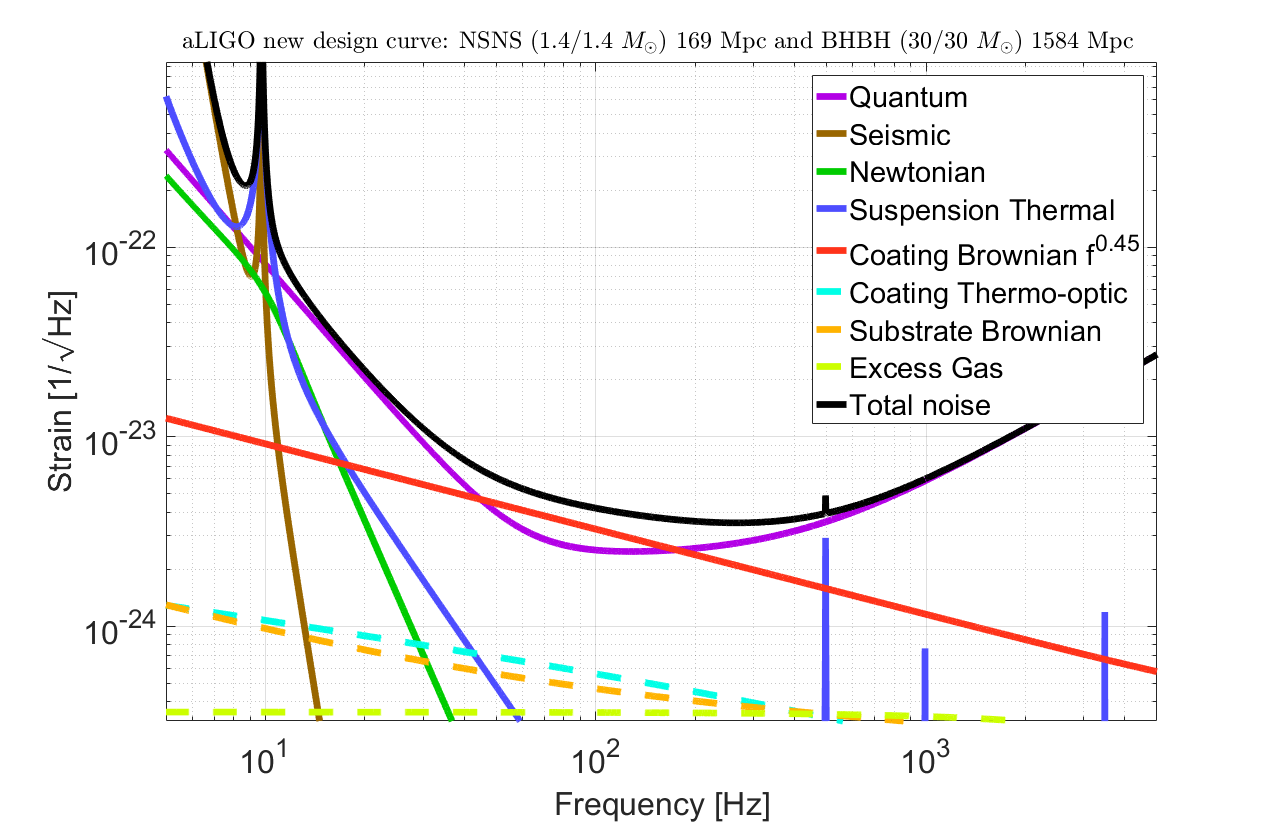
\includegraphics[width=\textwidth]{aLIGO_newDesign.png}
\label{fig:ALIGOSensitivity}
\caption{Advanced LIGO Noise budget from LIGO DCC T1800044-v4}
\end{figure}



At low frequencies, the sensitivity of current detectors is limited by a variety of noise sources. The ground seismic couples to the mirrors through the seismic isolation platforms and the suspensions.The seismic isolation concepts currently used are expandable and then sufficient for the next generation of detectors. Gravity gradient noise already plays a limiting role in today's detectors at times with increased seismic. Since there are no concepts to prevent or reduce the Newtonian coupling of seismic ground motion to the mirrors, the solution can only lie in a reduction of the ground motion itself or in a measurement and subsequent subtraction of the contributions. Suspension thermal noise, quantum radiation pressure noise, scattered light noise, alignment noise, and a variety of other not yet determined noise sources contribute to the total noise budget in the low-frequency range.
In the high frequency range the sensitivity can be improved by increasing the circulating light power in the interferometer arms and by using squeezed light with a high squeezing level. Both approaches put extreme demands on the optics. Increasing the laser power in the interferometer arms requires extremely low absorption, as due to local absorption of laser light and heating of the optics thermal effects could otherwise negatively affect the performance. Thermal compensation systems will have to be improved to reach the goals of future detectors. Increased light power also increases quantum radiation pressure noise. Due to the higher susceptibility of the mirrors to forces at low frequencies, radiation pressure noise is particularly effective in the low-frequency range. This can be counteracted on the one hand by increased mirror masses, and by frequency-dependent squeezing on the other. Increasing the squeezing level requires extremely low-loss optics, both in the interferometer arms and at the detection port, i.e. between the squeezed-light source, the interferometer, and the photodetector. The optical methods necessary for the rotation of the squeezing ellipse are not yet mature, both with regard to the technical implementation and control methods to be used. High light power in the interferometer arms can lead to parametric instabilities. These will already play an important role in the final stage of the current advanced detectors. The suppression mechanisms, e.g. with resonant dampers, probably need to be further improved to enable the higher light outputs in the next generation of detectors.
In the mid frequency range coating thermal noise becomes dominant over quantum noise.

\clearpage
\section{Facilities and Infrastructures}
\subsection{Current State of the Art}
\subsection{Requirements}
\subsubsection{3G initial}
\subsubsection{future}
\subsection{Pathways and required facilities}
\subsection{Type of collaboration required:  small/large}
\subsection{Suggested mechanisms}
\subsection{Impact/relation to 2G and upgrades}

\clearpage
\section{Core Optics}
\subsection{Current State of the Art}
\subsection{Requirements}
\subsubsection{3G initial}
\subsubsection{future}
\subsection{Pathways and required facilities}
\subsection{Type of collaboration required:  small/large}
\subsection{Suggested mechanisms}
\subsection{Impact/relation to 2G and upgrades}

\clearpage
\section{Coatings}
\label{sec:coatingsintro}
Optical Interference Coatings (OIC) are used in all optics of an interferometer but those deposited on the mirrors of the Fabry-Perot cavities are need to have the highest optical and mechanical performance. OIC are used to produce High Reflecting (HR) or Anti Reflecting (AR) surfaces. The transmission have to be specified over multiple wavelengths depending on the control scheme adopted by the detector. \\

The optical properties of the OIC that are relevant for a GW detectors are: Transmission $T(\lambda)$; absorption $\alpha(\lambda)$; Total Integrated Scatter (TIS); Bidirectional Reflectance Distribution Function (BRDF); wave form distortion; density of point defects. All these parameters need to have a specific uniformity over the optics surface. \\
The mechanical properties relevant for a GW detector are: mechanical loss angle $\phi$ for each elastic constant; the elastic constants; the internal stress $\sigma$; the adhesion to the substrate; thermal expansion coefficients; thermo elastic coefficients. Mechanical properties uniformity follow that of the optical properties.\\ 

Three main technologies are possible:\\
a) amorphous materials; \\
b) crystalline materials; \\
c) nano structured surfaces (coating-free optics). \\

New type of coatings are required for 3 potential wavelengths (1064 nm, 1550 nm and 2 $\mu$m), for 3 temperature ranges (room temperature, 120 K and below 20 K), for 3 different substrates (silica, sapphire and silicon) and for diameters ranging between 35 cm and 60 cm. \\

R\&D activities on materials, that are concentrated mostly on mechanical losses and absorption, have to go in parallel with the development of the deposition technology that should take care of all the other optical and mechanical parameters and that guaranties the uniformity of optical performance on large diameters.

There are 4 large areas of development in the coating research: Metrology, Materials, Deposition Technology and Fundamental Processes. In the following table a summary of the various research lines is provided:
%
\begin{longtable}{|p{0.25\textwidth}|p{0.3\textwidth}|p{0.45\textwidth}|}
\caption{Bla bla\label{tab:characterization}} \\
\hline\hline
\endfirsthead
\caption[]{(continued)}\\
\hline\hline
\endhead
{\sc Metrology} & Thermomechanical & Elastic Constants \\\cline{3-3}
 & & Internal stress \\\cline{3-3}
 & & Thermal coefficients \\\cline{2-3}
 & Mechanical Loss & Clamped systems \\\cline{3-3}
 & & Nodal systems \\\cline{3-3}
 & & Suspended systems \\\cline{2-3}
 & TN measurements & AF cantilevers \\\cline{3-3}
 & & Doubble paddle \\\cline{3-3}
 & & On mirrors \\\cline{2-3}
 & Optical characterization & Complex indeces \\\cline{3-3}
 & & Thermal coefficients \\\cline{3-3}
 & & Scattering \\\cline{3-3}
 & & Point defects statistics\\\hline\hline 
{\sc Materials} & Amorphous & Oxides \\\cline{3-3}
 & & Nitrides \\\cline{3-3}
 & & Fluorides \\\cline{3-3}
 & & Silicon \\\cline{3-3}
 & & Co-sputtered alloys \\\cline{3-3}
 & & Nano layered alloys \\\cline{2-3}
 & Crystallines & AlGaAs \\\cline{3-3}
 & & AlGaP \\\cline{3-3}
 & & AlGaN \\\cline{2-3}
 & Nano structured & On silicon \\\hline\hline
{\sc Deposition} & Amorphous & Uniformity \\\cline{3-3}
{\sc Technology} & & Parameters optimization \\\cline{3-3}
 & & Poit defect/scatterer reduction \\\cline{3-3}
 & & Post-deposition corrective coatings \\\cline{3-3}
 & & Elevated temperature deposition \\\cline{3-3}
 & & Annealing \\\cline{3-3}
 & & Nano layered structures \\\cline{2-3}
 & Crystallines & Uniformity \\\cline{3-3}
 & & Parameters optimization \\\cline{3-3}
 & & Point defect reduction \\\cline{3-3}
 & & Coatings transfert \\\cline{3-3}
 & & Adhesion \\\hline\hline
{\sc Fundamental} & Amorphous & Ultrastable glasses \\\cline{3-3}
{\sc Processes} & & Deposition processes \\\cline{3-3}
 & & Correlation loss-structure \\\cline{3-3}
 & & Correlation absorption-structure \\\cline{3-3}
 & & Role of contaminants \\\cline{2-3}
 & Crystallines & Dislocations \\\cline{3-3}
 & & Role of contaminants \\\cline{3-3}
 & & Effect of stress \\\cline{3-3}
 & & Mechanical losses from bonding \\\hline\hline
\end{longtable}
%
\subsection{Current State of the Art}
The materials used in the Advanced detectors have the following reference values for losses~\cite{Granata_2016} $\phi$ and extintion coefficient~\cite{Pinard_2017} $\kappa$ (it is linked to the attenuation through the relation $\alpha = 4\pi\,\kappa\,d/\lambda$ where $d$ is the thickness): \\
%
\begin{center}
\begin{tabular}{l|c|c|c}
            & $\phi$ & $\kappa$ & n \\ \hline
 SiO$_2$                 & $4.5\times 10^{-5}$ & $10^{-8}$        & 1.442  \\ \hline
 TiO$_2\,$Ta$_2$O$_5$    & $2.4\times 10^{-4}$ & $2\times 10^{-8}$ & 2.07  \\ \hline
\end{tabular}
\end{center}
%

%
\begin{minipage}{0.35\textwidth}
\end{minipage}\hfill
\begin{minipage}{0.6\textwidth}
\vspace{-0.cm}
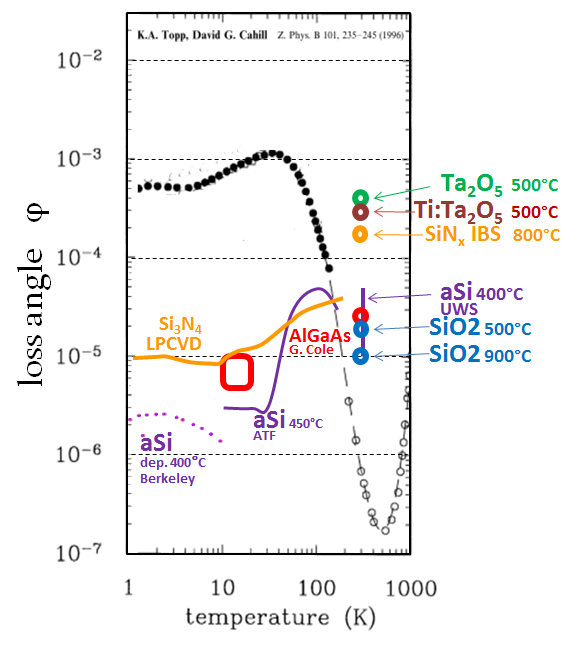
\includegraphics[width=\textwidth]{Figures/Status_coatings.png} \label{fig:coatinglosstatus}
\vspace{-0.5cm}
\captionof{figure}{Mechanical losses of the materials used in the Advanced detector and of some of the most promising materials. The measurements were done in the acoustic band.} \vspace{0.2cm}
\end{minipage}
%
\subsection{Requirements}
\subsubsection{3G initial}
\subsubsection{future}
\subsection{Pathways and required facilities}
\subsection{Type of collaboration required:  small/large}
\subsection{Suggested mechanisms}
\subsection{Impact/relation to 2G and upgrades}
\clearpage
\section{Cryogenics}
\label{s:Cryogenics}
A feature of most designs for future interferometers, is the 
cryogenic~\footnote{which we define here to be less than 123\,K; the range from 80\,--\,123\,K may be considered as "high temperature cryogenics"} operation of the test mass mirrors\cite{ET, Voyager}.

In the GW field, there is a long history of using cryogenic resonant mass detectors\cite{coldBars}, as well as the recent operation of the CLIO and KAGRA interferometers in Japan.

\paragraph{Thermal Noise}\mbox{}\\
The primary benefit of low temperature operation of the mirrors is through the reduced thermal noise:
\begin{itemize}
\item Brownian noise of mirror substrate
\item Brownian noise of mirror coating
\item thermo-optic (thermo-elastic and thermo-refractive) noise
\end{itemize}
The relation between the dissipation and the power spectrum of the noise is described by Callen's Fluctuation-Dissipation Theorem~\cite{CaWe1951, Kubo:FDT, Callen:1959}:
\begin{equation}
S_x(f) = \frac{k_B T}{\pi^2 f^2} \left| Re \big[ Y(f) \big]\right|
\label{eq:FDT}
\end{equation}
and so we see that the displacement noise, $x(f)$, scales as $\sqrt{T}$. More significantly, many of the material properties of mirror substrates (e.g. sapphire and silicon) and coatings (e.g. GaAs, GaP, $\alpha$-Si), scale in a favorable way with decreasing temperature. This makes the improvement in the noise substantially larger than the naive $\sqrt{T}$ scaling.

\paragraph{Robust Operation}\mbox{}\\
In addition to the noise improvement, there are a number of operational issues affected by a low temperature environment:
\begin{enumerate}
\item Increased thermal conductivity in crystalline substrates; this dramatically reduced the thermal gradients in the mirror, and thereby, the induced wavefront distortions due to thermo-elastic deformations of the mirror surface and thermo-refractive lensing in the substrate bulk.

\item zero thermal expansion in silicon at 18 and 123\,K

\item ???
\end{enumerate}



\subsection{Current State of the Art}
\begin{itemize}
\item cryogenic bars
\item CLIO
\item KAGRA
\item silicon Fabry-Perot cavities for atomic clocks (JILA, PTB)
\end{itemize}
\subsection{Requirements}
\subsubsection{3G initial}
\subsubsection{future}
\subsection{Pathways and required facilities}
What is needed to make a useful prototype?

What requirements on these prototypes?
\subsection{Type of collaboration required:  small/large}
\begin{enumerate}
\item 
\end{enumerate}
\subsection{Suggested mechanisms}

\subsection{Impact/relation to 2G and upgrades}



\clearpage
\section{Newtonian Noise}
\subsection{Current State of the Art}

\paragraph{Mitigation of atmospheric NN}
\begin{itemize}
\item Achieved below 2mHz in gravimeters using pressure sensors
\item NN spectra calculated based on highly-simplified models
\item Correlation studies between microphones carried out at Virgo
\end{itemize}

\paragraph{Mitigation of seismic NN}
\begin{itemize}
\item Achieved factor 1000 suppression of seismic signals in seismometers with underground array at Homestake
\item Achieved factor close to 100 suppression of seismic signals in seismometers with surface array at Hanford
\item Achieved factor >10 suppression of tilt signal in cBRS tiltmeter with surface array at Hanford
\item Analytical modeling of NN completed
\item Analytical modeling and numerical optimization of NN cancellation almost complete (missing the case of NN cancellation in underground arrays)
\end{itemize}

\paragraph{Site selection targets}
\begin{itemize}
\item Ambient seismic noise levels mostly understood from world-wide studies of impact of geology, distance to major cities, and coast
\item Some studies of geology made at existing detector sites and at Homestake
\item Seismic scattering from topography studied in linear order and only to obtain scattering coefficients
\end{itemize}

\paragraph{Infrastructure}
\begin{itemize}
\item Sound and seismic noise between about 5Hz and 50Hz are dominated by sources part of LIGO/Virgo infrastructure (e.g., ventilation) 
\item Stronger ground tilt is sometimes produced by wind pushing on buildings (problem clearly identified at LIGO sites); wind can also produce seismic noise at higher frequencies when interacting with rough surface topography
\end{itemize}

\subsection{Requirements}
\subsubsection{3G initial - surface}
\paragraph{Mitigation of atmospheric NN}
\begin{itemize}
\item Numerical simulations of atmospheric density perturbations
\item Analytical models of sound NN in terms of correlation functions (i.e., going beyond the plane-wave approximation)
\end{itemize}

\paragraph{Site selection targets}
\begin{itemize}
\item Investigate the impact of seismic scattering on NN cancellation
\end{itemize}

\paragraph{Infrastructure}
\begin{itemize}
\item Develop plans for low-noise detector infrastructure (with respect to sound and seismic disturbances)
\item Develop plans to avoid wind tilt at surface detectors
\end{itemize}

\subsubsection{3G initial - underground}
\paragraph{Mitigation of seismic NN}
\begin{itemize}
\item Analytic models of seismic NN from body waves in terms of correlation functions
\item Based on results from first item, calculate optimal underground arrays for cancellation
\end{itemize}

\paragraph{Mitigation of atmospheric NN}
\begin{itemize}
\item Investigate suppression of atmospheric NN as a function of detector depth using more realistic atmospheric models
\end{itemize}

\paragraph{Site selection}
\begin{itemize}
\item Investigate the impact of seismic scattering on NN cancellation
\end{itemize}

\paragraph{Infrastructure}
\begin{itemize}
\item Develop plans for low-noise detector infrastructure (with respect to sound and seismic disturbances)
\end{itemize}

\subsubsection{Future - surface}
\paragraph{Mitigation of atmospheric NN}
\begin{itemize}
\item Development of suitable instrumentation (e.g., LIDAR, effective wind shields for microphones) for NN cancellation
\end{itemize}

\paragraph{Site selection targets}
\begin{itemize}
\item Investigate the impact of seismic scattering on NN cancellation
\end{itemize}

\subsubsection{Future - underground}
\paragraph{Site selection targets}
\begin{itemize}
\item Investigate the impact of seismic scattering on NN cancellation
\end{itemize}

\subsection{Pathways and required facilities}
\subsection{Type of collaboration required:  small/large}
\subsection{Suggested mechanisms}
\subsection{Impact/relation to 2G and upgrades}
\clearpage
\section{Suspensions and Seismic Isolation Systems}
In this section we discuss suspensions and isolation systems for 3rd generation detectors. We have chosen to split our discussion into four areas: suspensions (especially the final stage), isolation, damping and control, and interface with cryogenics. The last two areas have overlap with the Simulation and Controls section and the Cryogenics section.
\subsection{Current State of the Art}
\subsubsection{Suspensions}
The use of fused silica fibers is a well-established technique for the final stage of the suspension of fused silica test masses, leading to a monolithic suspension.  Currently there are three detectors operating with room temperature fused silica suspensions: Advanced LIGO, Advanced Virgo and GEO600. Research is ongoing on silica within these collaborations.
The Kagra project is pursuing the use of cryogenic sapphire suspensions ( i.e. sapphire fibres supporting a sapphire test mass) working at ~20K. First operation of Kagra with its cooled sapphire suspensions is expected in 2019.
Research on sapphire is underway at Kagra as well as Glasgow, Perugia and KEK.
Application of silicon for future suspensions in GW detectors is under study in Glasgow, Perugia, KEK, Caltech and ANU.

\subsubsection{Isolation}
\subsubsection{Damping and Control}
\subsubsection{Interface with Cryogenics}



\subsection{Requirements, challenges and current/planned R \& D}

Suspension thermal noise and residual seismic noise are two of the dominant noise sources which limit the low frequency performance and define the low-frequency cut-off for ground based gravitational wave detectors. Thus the requirements of the suspension and isolation systems are to a great extent set by what the target low end of the operating frequency band is chosen to be, as well as by the intrinsic seismic levels of the chosen sites.

\subsubsection{Suspensions}

\subsubsubsection{Silica suspensions}
The use of fused silica is a well-established technique in both aLIGO and AdVIRGO,  and Perugia/EGO/VIRGO and Glasgow/aLIGO already have significant expertise. For future detectors at room temperature  we will aim to further reduce the suspension thermal noise. This is likely to involve suspension of heavy mirrors, up to several hundred kg, making the fibers as long as practicable, and making them relatively thinner to push down the bounce modes and push up the violin modes.  Ensuring robust techniques are available to handle the heavier masses will be an engineering challenge.
 
Moving to larger test masses will require rescaling the thermoelastic cancellation region to an appropriate diameter ref1. Pushing to lower bounce mode and higher violin mode frequencies will require a thinner central diameter fibre. This could result in operation at higher stress than currently used - around 1.2GPa-1.5GPa refs2,3. This will require some robustness testing to ensure suitably strong fibres for the detector lifetime (see ref4 for a general overview of suspension thermal noise reduction). Fused silica typically has a strength of 4-5GPa refs5,6.

Upgraded and enhanced silica fibre pulling/welding machines will be required to  pull the longer fibres and to weld from thicker stock material. Utilising thicker stock will reduce the loss component due to the weld and provide further improvement in the suspension thermal noise ref8. 

Pristine silica fibers are intrinsically strong, but need careful handling as well as protection from being accidentally touched. AdVirgo and aLIGO have experienced fiber breakages at some stage during assembly, installation or operation. Minimising the risk of touching, via well engineered installation tooling, is important to reduce downtime and should be taken into consideration in any revised suspension design, assembly and installation steps. AdVirgo has adopted a suspension solution that has fibers with two anchors, one at each end, to simplify the process of the removal and replacement of fibers. (see ref7). In aLIGO, fibers can be cut off at the ears on the mirror and new fibers welded in. Depending on the circumstances, in both designs there may be enough release of energy that the ears on the mirror could become too damaged to re-use without rework. Thus having spare mirrors ready is advantageous. 

\subsubsubsection{Sapphire and silicon suspensions}
There are several challenges involved in going to cryogenic temperatures, where silicon or sapphire are the materials of choice.
Suspending heavy mirrors with thick fibers/ribbons (for heat extraction) will need a smart design to soften the vertical and horizontal modes. Selection of material depends on the possibility to bond the suspension elements to the test masses made of the same or different material ref10. A significant challenge with 20K operation is the need to extract any deposited power via the fibres, which in turn drives their cross sectional area and vertical stiffness. Operation at ~120K is less challenging for heat extraction.

Cooling time is also a potential issue, as the timeline to commission such a detector may be driven by the several weeks to cool/warm up between vents. Currently there are efforts to work on mechanical heat links that can be removed. A cooling exchange gas is also a possibility, although may not used due to concerns about residual vacuum level.

The challenges above are common for sapphire/silicon. Sapphire as a material is transparent so can utilise traditional wavelengths. However, polishing/figuring and fabrication of fibres can be challenging due to material hardness. Laser heated pedestal growth, micro-pull down or machining (e.g. IMPEX) are possible techniques to fabricate fibres.

Silicon is a more standard material but requires 1500nm or greater wavelength. Material is more readily available in large sizes although the challenge will be getting sufficient purity. Fibre fabrication is at an early stage, although laser heated pedestal growth, micro-pull down or etching from wafers look possible.

The work of KAGRA is ground-breaking, leading to the first full stage sapphire suspensions operating at low temperature. The community will have a much better feel of where effort needs to be applied, but this will likely be in the area of sapphire/silicon fibre fabrication and testing (thermal conductivity, mechanical loss). Springs also need to be developed for the final stage suspensions at 20K as the vertical mode is high frequency and in-band.

A full design needs to be tested (KAGRA is pushing in this direction), but bonding, thermal extraction and losses need to be assessed/modelled. Moveable earthquake stops are probably needed to account for thermal expansion. A small scale (kg or larger) silicon prototype would be a valuable addition to the field to properly assess material losses (ref11).

Excess losses like clamping or bonding losses need to be studied with care. The challenge is to have a suspension dissipation dominated by the material thermal noise and not by the thermoelastic or other losses. Dissipation at the level of upper and lower clamps, thermoelastic losses for various geometries, surface losses (in case of geometries with large S/V), and bonding loss all need study.(ref11)

It is useful to note that typically it takes 10-15 years to get the hardware from prototype-interferometer, so prototypes are an essential step in the near future.

The fabrication methods for silicon and sapphire suspension fibers is an area which requires significant research. The way to assemble and/or to produce fibers/ribbons with different geometries is demanding. The various geometries will influence the way to clamp and assemble the whole suspension. For sapphire a laser heated pedestal growth, micro-pull down or direct machining will lead to circular cross section fibres. Some research focussed on fabrication/modelling would be beneficial.

For silicon, laser heated pedestal growth will lead to circular fibres, while micro-pull-down techniques (ref17) can give circular or ribbon geometries. Direct etching from a wafer would give ribbons. Rectangular fibres have the challenge that the energy leakage into the neck is larger, unless the geometry can be flared out quickly, and this can lead to larger loss due to energy deposition in the bond region ref18.

\subsubsubsection{Bonding}

Hydroxy-catalysis bonding (HCB) [24] is well known and has been used in GEO600, Virgo+, AdLigo, AdVirgo and Kagra for assembling monolithic suspensions.  It appears to work as expected in the present detectors, both at room temperature and cryogenics [25]. The strength, quality and losses have been measured for SiO2-SiO2, Al2O3-Al2O3 and Si-Si (refs22,23).   There is some fine tuning which could be investigated regarding the use of HCB, given small differences in the techniques used in Virgo and LSC, but common tests are already foreseen to establish general shared rules for the best results for application to 3G detectors.

Gallium bonding at the present time has been used in Kagra to connect the nail heads of the fibers to the upper Sapphire springs and to the lower mirror ears but still needs to be verified in working conditions,  More research is needed on the Ga-bonding, for example to  investigate the dissipation levels.  Different connecting materials such as indium are also of interest ref24, ref26). 

In general the quality of the bonding depends mainly on the polishing of the surfaces and on the mechanical precision of the components to be connected. Thus investigation of the assembly structures is required. To develop a very low dissipation suspension, precision in positioning the various components is important, and this is even more urgent in case of cryogenic suspensions where the bonding represents a discontinuity to the thermal flux and the mechanical tolerances are lower because of the rigidities of the system itself.

\subsubsubsection{Modelling}


Modelling of suspensions are important for understanding overall behaviour. Various groups have carried out simulations and modelling including dynamics of fiber suspensions (ref19) and violin mode splitting and long term stability, which ultimately feeds back into control of these modes (ref9). FEA analysis is an important tool as a cross check to design the best strategy to produce and realize the lower stage suspension. The losses and the heat fluxes can be simulated as well, even if the parameters need to be verified experimentally. A complete FEA with the various geometries, losses and thermal parameters is demanding. Linking the FEA analysis of the lower suspension stage with the codes used to estimate interferometer performance (e.g. GWINC) is of value.

Further activities which focus on modelling glitches in the detector will also be beneficial as instruments push to better strain sensitivity at lower frequencies (ref20).

\subsubsubsection{Upper Stages of Suspensions}
The work descibed above has focussed on the final stage of a suspension, i.e. the stage directly supporting the test mass. However consideration should also be put into the maraging steel blade springs and metal components at the upper stage(s) of the suspension, to ensure they do not limit thermal noise performance of the final stage. For example research into alternative materials for the blades, with lower loss than maraging steel, is an area worth pursuing. Kagra already incorporate sapphire springs at their final stage. Silicon is another material which can be considered. The challenges for using these materials include achieving a robust design with high breaking stress. Work on protective coatings, mechanical loss and thermal conductivity also need to be pursued.

\subsubsection{Isolation}

Some topics.

How much isolation (and how many stages required) will depend on site chosen, target sensitivity and and low-frequency cut-off. Overall height also affected by these considerations.

Need increased vertical isolation for longer arm lengths (increased coupling).

Combination of active and passive stages to be determined.

Materials/design compatible with low temperature if needed, e.g. passive damping materials for low T use, heat extraction.   

Isolation techniques for diffused light reduction.       



\subsubsection{Damping and Control}

Probbaly remove this section - covered elsewhere.

\subsubsection{Interface with Cryogenics}

Probbaly remove this section - covered elsewhere.

Here are some notes which Norna received concerning cryogenics and suspensions - to be combined with other input, moved elsewhere.

Heat conduction
Challenge
Maximise the heat extraction is the main condition for developing a cryogenic suspension. The suspensions will work better if the discontinuities (i.e. geometrical constraints, bondings) will be removed or as less as possible. The choice of the material and the best suspension configuration will be defined. The cryogenic suspension is by definition ‘out of thermal equilibrium’ and this needs to be evaluated correctly.

Cooling time is also a potential issue, as the timeline to commission such a detector maybe driven by the several weeks to cool/warm up between vents. Currently there are efforts to work on mechanical heat links that can be removed. A cooling exchange gas is also a possibility, although may not used due to concerns about residual vacuum level.

State of the art
The only cryogenic complete suspension has been realized for Kagra [21]. On our point of view a careful analysis needs to start from that one.
Research needed
The research on the various components that form the whole suspension is important as well as all the interconnections like the clampings or the bondings. 

Bibliography

[21] R Kumar et al 2016 J. Phys.: Conf. Ser. 716 012017

\subsection{Pathways and required facilities}
Prototypes are needed to test suspension/seismic isolation designs. 
\subsection{Type of collaboration required:  small/large}
No large collaborations are envisioned. 
\subsection{Suggested mechanisms}
Encourage participation in existing meetings (GWADW). 
\subsection{Impact/relation to 2G and upgrades}
2G facilities or upgrades to those can serve as test beds for 3G ideas. 

refs (to be moved).

1 Experimental results for nulling the effective thermal expansion coefficient of fused silica fibres under a static stress. Classical and Quantum Gravity, 31(6), 065010. (doi:10.1088/0264-9381/31/6/065010)

2 Heptonstall, A. et al. (2014) Enhanced characteristics of fused silica fibers using laser polishing. Classical and Quantum Gravity, 31(10), p. 105006. (doi:10.1088/0264-9381/31/10/105006)
Bell, C. J., Reid, S., Faller, J., Hammond, G. D., Hough, J., Martin, I. W., Rowan, S. and Tokmakov, K. V. (2014) 

3 Aisa, D. et al. (2016) The Advanced Virgo monolithic fused silica suspension. Nuclear Instruments and Methods in Physics Research Section A-accelerators spectrometers detectors and associated equipment, 824

4 Hammond, G., Hild, S. and Pitkin, M. (2014) Advanced technologies for future ground-based, laser-interferometric gravitational wave detectors. Journal of Modern Optics, 61(Sup. 1), S10-S45. (doi:10.1080/09500340.2014.920934)

5 Tokmakov, K.V., Cumming, A., Hough, J., Jones, R., Kumar, R., Reid, S., Rowan, S., Lockerbie, N.A., Wanner, A. and Hammond, G., (2012) A study of the fracture mechanisms in pristine silica fibres utilising high speed imaging techniques. Journal of Non-Crystalline Solids, 358(14), pp. 1699-1709. 
(doi:10.1016/j.jnoncrysol.2012.05.005)

6 Amico, P., Bosi, L., Carbone, L., Gammaitoni, L., Marchesoni, F., Punturo, M., Travasso, F., Vocca, H. (2002) Monolithic fused silica suspension for the Virgo gravitational waves detector. Review of Scientific Instruments, 73(9). (DOI: 10.1063/1.1499540)

7 Travasso, F. on behalf of Virgo Collaboration (2018) Status of the Monolithic Suspensions for Advanced Virgo. IOP Conf. Series: Journal of Physics: Conf. Series 957 (2018) 012012  (doi:10.1088/1742-6596/957/1/012012)

8 Hammond, G.D., Cumming, A.V., Hough, J., Kumar, R., Tokmakov, K., Reid, S. and Rowan, S. (2012) Reducing the suspension thermal noise of advanced gravitational wave detectors. Classical and Quantum Gravity, 29(12), Art. 124009. (doi:10.1088/0264-9381/29/12/124009)

9 https://dcc.ligo.org/LIGO-G1700038

10 Cumming, A.V. et al. (2013) Silicon mirror suspensions for gravitational wave detectors. Classical and Quantum Gravity, 31(2), 025017. (doi:10.1088/0264-9381/31/2/025017)

11 Nawrodt, R. et al. (2013) Investigation of mechanical losses of thin silicon flexures at low temperatures. Classical and Quantum Gravity, 30(11), p. 115008. (doi:10.1088/0264-9381/30/11/115008)

12 K. Haughian et al., Mechanical loss of a hydroxide catalysis bond between sapphire substrates and its effect on the sensitivity of future gravitational wave detectors, Phys. Rev. D 94, 082003 – Published 12 October 2016

13 Alshourbagy, M. et al. (2006) Measurement of the thermoelastic properties of crystalline Si fibres. Classical and Quantum Gravity 23(8) (doi.org/10.1088/0264-9381/23/8/S35)

14 Alshourbagy, M. et al. (2006) First characterization of silicon crystalline fibers produced with the mu-pulling technique for future gravitational wave detectors. Review of Scientific Instruments, 77(4) (doi.org/10.1063/1.2194486)

15 Amico, P., Bosi, L., Gammaitoni, L., Losurdo, G., Marchesoni, F., Mazzoni, M., Parisi, D., Punturo, M., Stanga, R., Toncelli, A., Tonelli, M., Travasso, F., Vetrano, F., Vocca, H. (2004) Monocrystalline fibres for low thermal noise suspension in advanced gravitational wave detectors. Classical and Quantum Gravity, 21(5) (doi.org/10.1088/0264-9381/21/5/094)

16 Cumming, A.V. et al. (2013) Silicon mirror suspensions for gravitational wave detectors. Classical and Quantum Gravity, 31(2), 025017. (doi:10.1088/0264-9381/31/2/025017)

17 www.infn.it/thesis/PDF/getfile.php?filename=781-Alshourbagy-dottorato.pdf

18 Cumming, A.V. et al. (2013) Silicon mirror suspensions for gravitational wave detectors. Classical and Quantum Gravity, 31(2), 025017. (doi:10.1088/0264-9381/31/2/025017)

19 Lorenzini, M., Cagnoli, G., Campagna, E., Cesarini, E., Losurdo, G., Martelli, F., Vetrano, F., Vicere', A. (2010) The dynamics of monolithic suspensions for advanced detectors: A 3-segment model. J. Phys.: Conf. Ser. 228. (doi.org/10.1088/1742-6596/228/1/012017)

20 https://dcc.ligo.org/LIGO-G1501237

21 R Kumar et al 2016 J. Phys.: Conf. Ser. 716 012017

22 Dari, A., Travasso, F., Vocca, H., Gammaitoni, L. (2010) Breaking strength tests on silicon and sapphire bondings for gravitational wave detectors. Classical and Quantum Gravity, 27(4). (doi.org/10.1088/0264-9381/27/4/045010)

23 Amico, P., Bosi, L., Carbone, L., Gammaitoni, L., Punturo, M., Travasso, F., Vocca, H. (2002) Fused silica suspension for the VIRGO optics: status and perspectives. Classical and Quantum Gravity, 19(7). (doi.org/10.1088/0264-9381/19/7/359)

24 van Veggel, A.-M. A. and Killow, C. J. (2014) Hydroxide catalysis bonding for astronomical instruments. Advanced Optical Technologies, 3(3), pp. 293-307. (doi:10.1515/aot-2014-0022)

25 K. Haughian et al., Mechanical loss of a hydroxide catalysis bond between sapphire substrates and its effect on the sensitivity of future gravitational wave detectors, Phys. Rev. D 94, 082003 – Published 12 October 2016

26 Hofmann, G. et al. (2015) Indium joints for cryogenic gravitational wave detectors. Classical and Quantum Gravity, 32(24), 245013. (doi:10.1088/0264-9381/32/24/245013)

27 Murray, P. G., Martin, I. W., Cunningham, L., Craig, K., Hammond, G. D., Hofmann, G., Hough, J., Nawrodt, R., Reifert, D. and Rowan, S. (2015) Low-temperature mechanical dissipation of thermally evaporated indium film for use in interferometric gravitational wave detectors. Classical and Quantum Gravity, 32(11), 115014. (doi:10.1088/0264-9381/32/11/115014)




\clearpage
\section{Light Sources}
{\color{blue} edited on 15 May by Benno\\
edited ... by ...}\\
This section is devoted to light sources for 3G IFOs. It includes the pre-stabilized high power lasers (PSL) and the squeezed light sources. It does NOT include filter cavities for frequency dependent squeezing quadrature rotation. 
\subsection{Current State of the Art}
\begin{itemize}
\item all advanced GWDs have problems with their lasers
\item several solutions are being tested: 200\,W class fiber amplifiers (AEI/LZH, MIT, Artemis) and coherently combined solid state amplifiers (AEI)
\item high power lasers demonstrated in lab
	\begin{itemize}
    \item 1064\,nm
    \item 1550\,nm
    \item $\rm 2\,\mu m$
	\end{itemize}
\item problem with durability
\item squeezed light sources 
\begin{itemize}
    \item 1064\,nm
    \item 1550\,nm
    \item $\rm 2\,\mu m$
	\end{itemize}
\end{itemize}

\subsection{Requirements and current/planned R\&D}
We analyzed available documentation and presentations on next generation gravitational wave detectors (GWDs) to extract requirements for the high power lasers and squeezers. In parallel the  R\&D currently performed within the worldwide gravitational wave (GW) community was identified by sending a questionnaire to 32 laser and sqeezing experts in all GW projects. The questionnaire asked for current and planned R\&D and for desired collaboration topics and coordination mechanisms. The findings are summarized in this sub section.
The requirements on the pre-stabilized high power laser and the squeezed light sources for 3rd generation GWDs do not seem to be well defined yet. The design of the Einstein Telescope (ET) as defined in the ET design study is build on a 500\,W laser at 1064\,nm in the spatial $\rm LG_{33}$ mode and a 3\,W laser at a wavelength of 1150\,nm in the fundamental Gaussian mode. Even though these are clear requirement, the ET design is currently re-evaluated. In particular the operation of the ET high power IFO in the spatial $\rm LG_{33}$ seems questionable. The current Cosmic Explore (CE) and LIGO Voyager (LV) designs are build on high power light sources with a power of 200\,W and a wavelength of 1550nm or longer for a small absorption coefficients for the light to be transmitted by Silicon test masses. The wavelength choice depends on several factors as e.g. available high power lasers, absorption of the bulk and the high reflective coatings of the test masses, scattering and the availability of photo detectors with high quantum efficiency. As information on several of these factors is missing, a final wavelength choice can not yet be made. Currently the wavelength of 1550\,nm and around $\rm 2\, \mu m $ are favored due to promising high power laser concepts for these wavelength. Hence R\&D on high power laser and squeezer for three different wavelength (1064\,nm, 1550\,nm and around $\rm 2\, \mu m $) has to be performed until the final operation wavelength are selected. All current 3G GWD designs are currently build on 10dB detected squeezing such that squeezed vacuum sources with squeezing levels of $> 15\,dB$ are required. No information on PSLs stability requirements for 3G GWD detectors could be found. As a 10 times better sensitivity is aimed for we assume that the power, frequency and beam jitter stability has to be a factor of 10 higher. Concerning the spatial and polarization purity we expect similar requirements as for the Advanced GWDs.
With the afore mentioned questionnaire we found, that the current or planned research of at least two groups covers the identified required research areas (see Fig. 
\begin{figure}[h]
% \centering
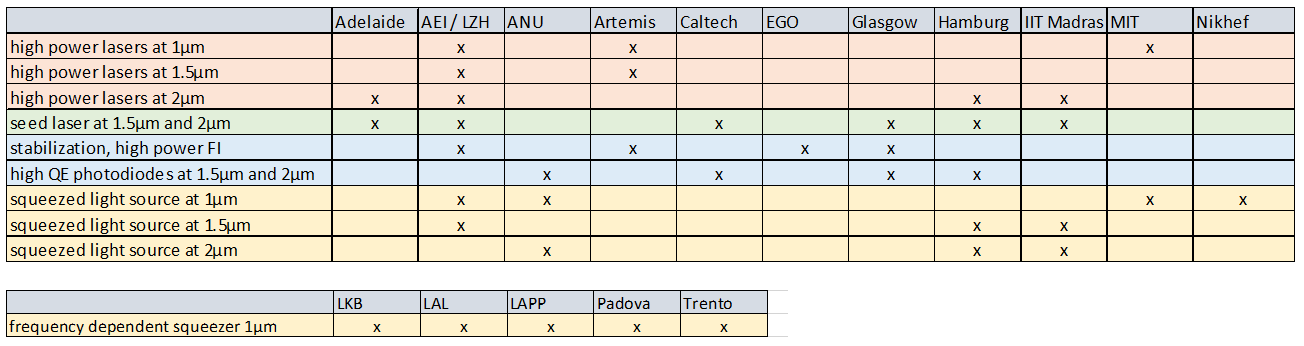
\includegraphics[scale=0.5]{Light_source_Fig1.png}
\caption{Current or planned R\&D on high power laser and squeezed vacuum sources}
\label{fig:LightSourceRD}
\end{figure}

% \subsubsection{3G initial}
% \subsubsection{future}
\subsection{Pathways and required facilities}
\subsubsection{laboratory prototypes}
Show that high power generation concepts works reliable, accept poor noise performance, missing diagnostic and actuators for stabilization
\subsubsection*{1064\,nm}
we assume reliability problem of 200\,W class fiber amplifier will be solved for Advanced detectors (current work at AEI/LZH, MIT and Artemis)\\
develop coherent combination techniques at 2x250W power level
\subsubsection*{1550\,nm}
assume AEI/LZH fiber amplifier development is successful
\subsubsection*{$\rm \bf 2\,\mu m$}
assume either Adelaide cryo HM or wavelength doubling of 1064\,nm in OPA is successful
\subsubsection*{stabilization}
develop stabilization concepts for all three wavelength adequate for free running noise and available actuators of laboratory PT developments
\subsubsection{engineering prototype}
after final wavelength selection transfer concepts to laser lab or company capable of designing and fabricating an engineering prototype that meets all requirements concerning power, noise performance, spatial and polarization purity, actuators with sufficient range and bandwidth, diagnostic\\
transfer engineering prototype to research lab for characterization and pre-stabilization\\
build several engineering prototypes for long-term/reliability tests
\subsection{Type of collaboration required:  small/large}
small, summarize results of questionnaire\\
once at engineering PT stage: synergy between projects requiring similar lasers (if possible avoid single supplier problem)

\subsection{Suggested mechanisms}
annual meetings, keep list of who does what,\\
team up of GWD projects and funding agencies in engineering PT stage
\subsection{Impact/relation to 2G and upgrades}
at 1064nm laser development for 2G and upgrades is in direct path to 3G and will serve as long-term test of some concepts

\clearpage
\section{Quantum Enhancements}
\subsection{Quantum Noise Reduction Techniques under consideration}
Quick overview of the most prominent quantum noise reduction techniques currently persued. Maybe this could be done in a separate explanation box rather 
than in the main text of the document?
\subsection{Current State of the Art}
\begin{itemize}
\item Dual-recycled, Fabry-Perot Michelson
\item Injection of squeezed light, obtaining about 4dB max
\item A+ and Advanced Virgo+ will test frequency dependent squeezing with short (300\,m) filtercavities, targetting 6dB effective squeezing.
\item Balanced Homodyne readout will be part of A+, allowing in principle to change readout quadrature.
\item Quick list of current losses for 1064nm: QE PDs, faraday isolators etc.
\end{itemize}
\subsection{Requirements}
Need to start here with a quick discussion on the relation of quantum noise 
and laser wavelength: To first order quantum noise reduction schemes are independent of wavelength so all the drivers for changing towards longer wavelength come from other noise sources.Hence in the following assume that each of the discussed quantum noise reduction techniques can be realised equally well for any laser wavelength. However, we need to keep in mind that there could 
be potential somestoppers, e.g. if it would turn out that there are no high 
quantum efficiency photo diodes available at 2 micron, which could lead for quantum noise considerations to rule out certain wavelengths.  
\subsubsection{3G initial}
\begin{itemize}
\item \textbf{Result driven: 10\,dB effective quantum noise reduction over 2G for frequencies at mid and high frequency, plus pushing the radiation pressure noise below a few Hertz.}
\item Current baselines: ET and CE designs are currently based on tuned (ET-HF and CE) or detuned (ET-LF) dual-recycled Fabry Perot Michelson interferometers, with frequency dependent squeezing created with km-scale filter cavities, combined with heavy test masses of the order 200\,kg to reduce radiation pressure noise at low frequencies. 
\item Alternative approaches: Several alternative approaches are currently researched which provide more cost effective ways to improve the same senstivity as the baselines mentioned above. Examples include conditional squeezing which uses an EPR measurement for generation of frequency dependent squeezed light and therefore removes the need for long baseline filtercavities; speedmeter interferometers which inherently surpress back action noise.     
\end{itemize}
\subsubsection{future}
No limit. The more reduction the merrier. (Obviously need some better words for this section. Might need to discuss within full committee what level of speculation/optyimism one should put in here to make it consident with the other sections?)
\subsection{Pathways and required facilities}
\begin{itemize}
\item Bench mark parameter set, for evaluation of different quantum noise reduction schemes. 
\item Deticated prototype test programmes for full interferometer schemes and low noise tests.
\item Table top tests of interferometer building blocks, such as low loss optics, high QE photo diodes. 
\end{itemize}
\subsection{Type of collaboration required:  small/large}
\begin{itemize}
\item From feedback we received from community, the key that is needed is not 
necessarily more collaboration (though this si also welcome), but rather more coordination, to make sure there are prototype experiments testing all the different promising configurations and we do not miss to develop one. 
\end{itemize}
\subsection{Suggested mechanisms}
\begin{itemize}
\item Community feedback asked for annual quantum noise workshop with special focus to bring together theorists and experimentalists. 
\item Prototype coordination (partly happening already via LSC MOUs). Which body would take this on to cover more than just LSC?
\end{itemize}
\subsection{Impact/relation to 2G and upgrades}
\begin{itemize}
\item 2G consolidates state of the art and test baseline scheme, i.e. frequency
dependent squeezing. 
\item Benefit for 3G programme for 2G: Potentially improved sensivity and faster commissioning plus risk reduction.
\end{itemize}
\clearpage
\section{Auxiliary Optics}
\subsection{Current State of the Art}
\subsubsection{Input optics}
\paragraph{Introduction}
In all the ground-based laser-interferometric gravitational wave detectors, the light which is injected into the main interferometer comes from high power lasers operating at 1064nm, with powers which could exceed 100 W (maximum 200W). Their frequency stability in the detection frequency band (10Hz-10kHz) is what you can find as the best in the world. Similarly, the relative intensity noise (RIN) of the laser beam is at the state of the art in laser power stabilization (2.10$^{-9}$/$\sqrt(Hz)$). Their spatial eigenmode is very close to an ideal Gaussian mode. In a first paragraph, we will give an overview of the function carried out by the Input optics.

\paragraph {Overview}

The Input Optics is the interface between the laser system and the Interferometer. It is also part of the Pre-stabilized laser. The whole system delivers a beam at the interferometer input port with the required power, geometrical shape, frequency and angular stability. An Electro Optic Modulation (EOM) system is providing the RF modulations needed for control and sensing purposes. The Input Mode Cleaner (IMC) cavity geometrically cleans the beam and reduces its amplitude and lateral fluctuation. The resonant IMC in conjunction with a reference cavity (RFC) are used to stabilize the laser frequency.
After the IMC some photodetectors provide the signal for intensity stabilization of the laser. An in-vacuum Faraday isolator prevents the light reflected by the interferometer goes back to the laser system and allows a simple extraction of this reflected beam. Finally, a mode matching telescope is used to properly match the beam on the Interferometer.

\paragraph {Wavelength and power handling}
In the first and second generation of GW detectors based on laser interferometers, the working wavelength is 1064nm which is produced by Nd:YAG solid state lasers. The power of the laser source in the first generation was of the order of a few tens of Watts which became a few hundred of Watts for the second generation. Up to now the detectors have been operated at a maximum of 50Watts injected in the interferometer but the plan is to reach 125Watts in the later developments of this generation. Due to the high power densities in the optical components such as the EOM system and the Faraday isolator, those devices has been specially developed for the Gravitational Wave detectors. 

\paragraph {Electro optic modulation system}
State of the art of the EOMs currently used will be given here.

\paragraph {Faraday isolators}
State of the art of the FIs currently used will be given here.

\paragraph {Input mode cleaner}
State of the art of the IMC cavities currently used will be given here.
Why Geo uses 2 IMCs?

\begin{table}[htp]
\begin{tabular}{@{}l c c c c c@{}}
Parameter & LIGO & Virgo & GEO & &Kagra\\
       &  &   &  IMC1  & IMC2 &  \\
\hline
Optical cavity length & 32.945 m & 286.845 m & 8 m & 8.1 m & 53.3m (TBC)\\
Free spectral range & 9,099,786 Hz & 1,045,137 Hz & 37.48 MHz & 37.12 MHz &\\
Radius of curvature of MC2 & 27.27 m & 185.1 m& & &\\
Flat mirror transmissivities & 6000 ppm & 2880 ppm & & & 6000 ppm \\
MC2 transmissivity & 5 ppm & 2.2 ppm & & &< 200ppm\\
Cavity Pole frequency & 8.72 kHz & 520 Hz & & & \\
\hline
\end{tabular}
\label{IMC cavities main parameters}
\end{table}

\paragraph{Mode matching telescope}
MMT will be described here and some references will be given.

\paragraph {Performances and issues}
In this paragraph we will describe the performances obtained (firstly underlining that GWs have been detected both with LIGO and Virgo). Then, we can write a few sentences on the beam jitter which represents one of the most annoying technical noises we can find at the level of the IO in the current generation. There are some possible mitigations (such as increasing beam jitter reduction in vacuum as underlined by Matt and proposed in LIGO (See Jitter Attenuation Cavity \url{https://dcc.ligo.org/LIGO-T1600595}))

\subsubsection{Output optics}
The output optics subsystem of interferometric GW detectors typically refers to all optics in the detection chain after the signal recycling mirror. In the advanced generation of detectors, this includes the beam steering optics, output Faraday isolator, output mode cleaner, and photodetectors. For squeezing enhanced detectors, the output optics includes all optics between the squeezing source and the main interferometer, as well as probably alignment sensing and control, a squeezing phase sensing and control scheme, and mode matching optics.
In A+, the near term upgrade to Advanced LIGO, this will also include the 300\,m filter cavity which is used to provide frequency dependent squeezing for sensitivity enhancement at all frequencies in the detection band. 

\paragraph {Output mode cleaner}
Advanced LIGO and Advanced Virgo both employ suspended in-vacuum 4-mirror output mode cleaner cavities (OMCs). 
These cavities are used for two primary purposes: to clean the spatial mode of the interferometer output beam (rejecting higher-order spatial modes which add shot noise but no signal), and to remove the rf sidebands from the light which reaches the phototdetectors which are used to read out the GW signal. OMCs are necessary for the DC readout scheme which has been in use since GEO600, enhanced LIGO and Virgo+ (fact check please)~\cite{dcreadout}. 
The output mode cleaner cavity should be designed such that the sidebands HG$_{00}$ mode and all higher-order modes are not co-resonant with the carrier frequency HG$_{00}$ mode. Scattered light in the OMC is also a serious concern. 
Add some more detail here on the aLIGO and AdVirgo OMCs. Anything for A+ or 3G OMCs?

\paragraph{Photodetectors}
The photodetectors which are currently used for the GW signal detection are all InGaAs detectors, which have been screened for high quantum efficiency at 1064\,nm. Most of the current R\&D into high-quantum efficiency is aimed at longer wavelengths. Some details here perhaps on where the aLIGO and AdVirgo PDs were sourced from. Who is working on high-QE PDs at 1550\,nm.

\paragraph{Balanced homodyne detection}
The LSC currently has a specific subgroup which has been tasked with developing the necessary designs and technology for implementing balanced homodyne detection (BHD) in the A+ interferometers. Balanced homodyne detection requires that the output light from the interferometer is interfered against a stable reference field. Adjusting the relative phase of the two fields allows to adjust the readout quadrature of the GW signal. In the currently used DC readout scheme carrier light from within the interferometer is used as the reference field, by slightly detuning the differential arm length (DARM) degree of freedom. In this scheme, however, the phase of the reference field cannot be adjusted against the GW signal field. The LSC BHD R\&D is coordinated through the LSC wiki page here: \url{https://wiki.ligo.org/AIC/BHD_A_plus}. Stefan Hild from the University of Glasgow is leading this effort. Any knowledge of efforts at AdVirgo to include BHD?

\paragraph{Filter cavities}
Filter cavities have been a topic of research within the GW community since they were demonstrated to effectively rotate the squeezing angle (or quadrature) of squeezed light reflected from the cavity in the frequency band around resonance~\cite{chelkowski}. Initial demonstrations were performed for squeezing at Fourier frequencies in the rf band, but in recent years frequency dependent squeezing with filter cavities was demonstrated in the audio frequency band~\cite{MITfiltercav}. Frequency dependent squeezing becomes necessary for GW detectors as the detectors become increasingly limited by quantum noise, both at the high frequency end of the measurement band (shot noise) and the low frequency end (quantum radiation pressure noise). Frequency independent squeezing can only improve one of these quantum noise effects, while exacerbating the other. The filter cavity must have a linewidth which is close to that of the core interferometer for GW signal sidebands. In the case of Advanced LIGO, this value is roughly 100\,Hz (fact check please). To make a filter cavity with such small linewidth, the cavity must either be extremely long, or extremely high finesse. In the high-finesse case, optical losses at the mirror surfaces become increasingly significant, leading to a degradation in the squeezing depth. It is an active topic of research in the community to determine the optimal filter cavity parameters with regards to length and finesse, although designs for A+ are being consolidated currently. Something about who is working on filter cavities here... 

\paragraph{Low-loss Faraday isolator}
The output Faraday isolator (OFI) is currently used to reject backscattered light from the photodetectors and OMC from re-entering the interferoemter. Optical losses in the OFI currently do not have a severe impact on the detector sensitivity, they simply degrade the signal by reducing the total amount of light reaching the photodetectors. In principle this can be compensated by simply using a larger DARM offset.
With the addition of squeezed light enhancement however, optical losses in the OFI becomes much more critical. In a squeezing enhanced interferometer, the OFI also serves a second purpose as the injection port for the squeezed light. The squeezed light passes through the OFI twice before reaching the photodetectors. Optical losses in the squeezing path reduce the effective squeezing severely, and if bad enough will actually make the quantum noise limited sensitivity worse than with no squeezing at all~\cite{dwyer}. Low-loss Faraday isolators is therefore seen throughout the community as a critical R\&D topic for output optics in the drive towards 3G sensitivities.

\subsubsection{Active wavefront control}
Active wavefront control (AWC) is a term which has been coined to cover the sensing and control of all beam mismatches and imperfections in the optical chain which are of a higher spatial frequency than simple misalignment. At the first order, this corresponds to spherical mode mismatches between the various beam and cavity eigenmodes. AWC also in principle includes higher-order wavefront distortions such as astigmatism, coma, trefoil and so on. In many cases, the spatial mode in the interferometer cavities is laser power-dependent, due to absorption in the substrates and coatings of the optics. In other cases mode mismatches result simply from imperfect placement of optics, or from fixed deviations of the optics from design specifications. Several different AWC technologies have been developed in order to manage the many different kinds of mode mismatches in the interferometers. We will give a brief description of these here.

\paragraph{Core optics thermal compensation}
\begin{itemize}
\item Ring heaters
\item CO$_{2}$ laser and compensation plates.
\item Projected heaters (CHROCC), SR3 heater at aLIGO etc.
\item anything else?
\end{itemize}
\paragraph{Input mode matching}
\begin{itemize}
\item UF/Syracuse thermal lens
\item backside heated mirror
\item anything else?
\end{itemize}

\paragraph{Output mode matching}
\begin{itemize}
\item UF/Syracuse thermal lens
\item backside heated mirror
\item anything else?
\item this is extra critical because of squeezing, losses etc.
\end{itemize}
\paragraph{Mismatch sensing}
\begin{itemize}
\item Phase camera
\item Hartman sensor
\item Bullseye sensor
\item Mode converter and QPD
\item Beam size jitter sensing
\end{itemize}
\subsubsection{Stray light control}
\paragraph{Baffles}
Something about what was done with baffling at aLIGO and AdVirgo. What worked well and what did not? What has already been earmarked for upgrades?

\paragraph{Optics}
What did we learn from aLIGO and AdVirgo about scattering from optics?

\subsubsection{Other auxiliary optics}

\paragraph{Optical levers}
\paragraph{Alignment sensing schemes}

\subsection{Requirements and current/planned R\&D}
\subsubsection{Survey of current R\&D}
A survey was conducted throughout research groups who are known to be working on, or have previously worked on auxiliary optics topics. The table shown in Fig.~\ref{fig:auxopticssurvey} shows the current status of the worldwide auxiliary optics R\&D, as informed by this survey. 
\begin{figure}[htb]
\centering
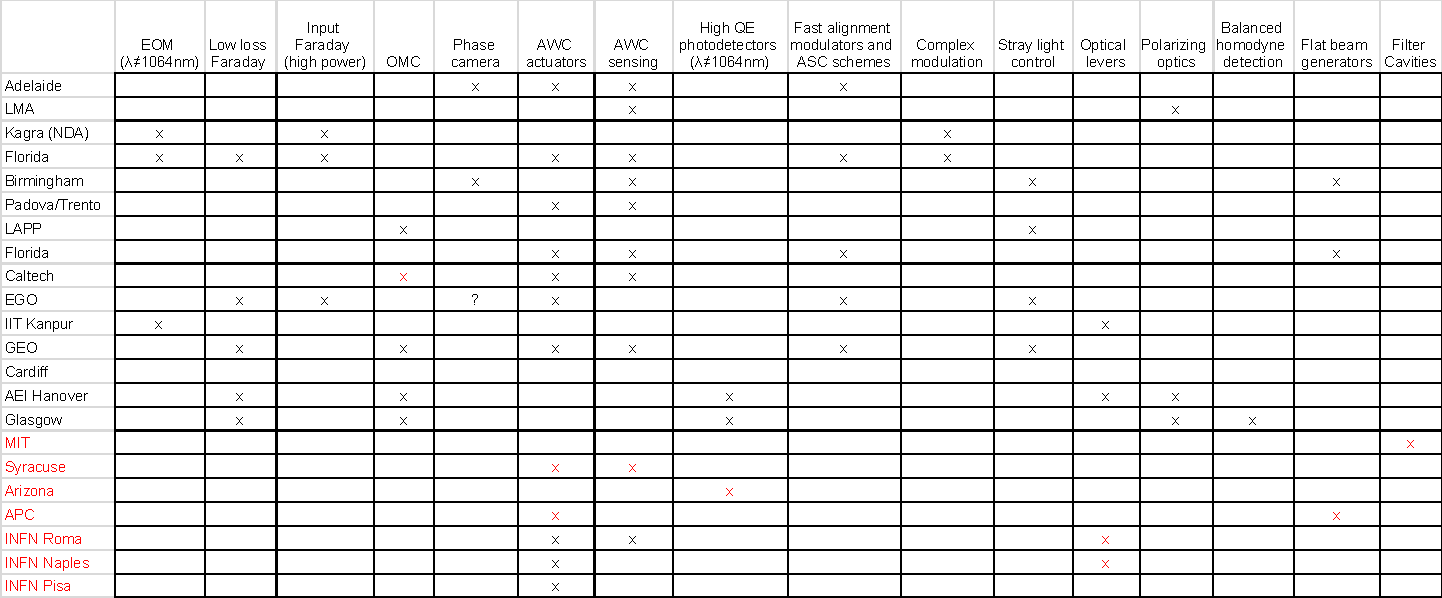
\includegraphics[scale=0.65]{Figures/auxopticssurvey.pdf}
\caption{The current status of global gravitational wave detector auxiliary optics R\&D, based on the responses to an email survey and the knowledge of subcommittee members.}\label{figauxopticsssurvey}
\end{figure}

The remainder of this section is subdivided into a discussion of the requirements for each auxiliary optics subcategory in the context of laser wavelengths between 1 and 1.55\,$\mu$m and 1.55\,$\mu$m and above. Where there is expected to be no major difference between the R\&D required for both wavelength ranges, the R\&D will be described in the section for the shorter wavelength range only. 

\subsubsection{1-1.55\,$\mu$m laser wavelength R\&D requirements}
\paragraph{Input optics}
In that wavelength range, we do not expect particular issues with respect to the 2G. The main issue might concern scattered light management and beam jitter mitigation.
We mostly rely the developments which have been made for the first and second generation of GW detectors at 1.064 $\mu$m. For 1.55$\mu$m, there will be for sure the need of R\&D on wavelength dependent optical devices such as the Faraday isolator especially if we want to work at very high power at 1.55$\mu$m. Some R\&D activities are already planned in several groups (IAP, UF and EGO) so we do not expect major issues on that point.
Below we just list the most important sub-parts of the IO.
\begin{itemize}
\item	High power Faraday isolator for 1 and 1.55 um R\&D on-going.
\item	EOMs. Seems to be under control but might be needed to think about RAM noise.
\item	Complex modulation - can be used to minimize am (better control of locking point offsets). R\&D ongoing.
\item	Fast alignment actuators. Alignment sensing and/or control. R\&D ongoing.
\item	Flat beam generators (LG modes etc.). Not much active research recently.
\item	Input mode cleaner and frequency stabilization scheme (not R\&D more related to design choices). 
\end{itemize}
\paragraph{Output optics}
The main point will consist in mitigating the scattered light which is harmful for the Interferometer sensitivities in the second generation of GW detector.
R\&D activity on OMC could be useful?
For what concerns the development of low-loss Faraday isolator for the squeezed light injection at 1$\mu$m, the situation seems well under control. A few groups are working on that topic (UF,AEI and EGO). Some good results have been obtained recently with the demonstration of sub percent loss Faraday isolators (see for example refLLFI). We can reasonably expect to get below 0.5\% for a single pass. If the losses have to be lower some particular effort will have to be devoted to that topic.\\ 
Filter cavity

refLLFI E. Genin and G. Pillant, Development of Low loss Faraday isolators at EGO, Presentation at LVC Sonoma meeting, March 2018, \url{https://dcc.ligo.org/DocDB/0150/G1800468/001/LowlossFIupdate_20032018_v2.pdf}

\paragraph{Active wavefront control}
At 1um we can base the TCS system on what has been used in the second generation GW detectors.
At 1.55$\mu$m, it could be required to change the actuation techniques if we change the test mass material. 
In general we expect that the requirements on mode matching and contrast defect become significantly more stringent for upgrades to the Advanced detectors, and for the 3G detectors. This is primarily because of the expected addition of squeezed light enhanced to the detectors. Mode mismatches in the core interferometer and the signal extraction chain can cause at best a reduction in the benefit of squeezing at certain frequencies (i.e. in the case of mode mismatch to a filter cavity), and at worst an effective optical loss 

\paragraph{Stray light mitigation}
The light absorption from the baffles is very dependent on the wavelength. So it is likely that what will work at 1um but not at 1.55 $\mu$m. R\&D will be required to find new materials suitable for 1.55$\mu$m.  

\paragraph{Other auxiliary optics}
{\bf Optical levers}
Increasing the length of the arm cavities can represent a problem from the optical levers point of view. A preliminary study should be done in order to understand the requirements on the suspended optics residual motion tolerated to be able to lock the arm cavities (40 km is quite long!).

{\bf Alignment sensing schemes}

{\bf Polarization optics}
In the case that a Sagnac-type interferometer is to be used for 3G detectors, one option will be a polarization based Sagnac

\subsubsection{1.55+\,$\mu$m laser wavelength R\&D requirements}
Above 1.55 $\mu$m and especially if we go to 2 or 2.1 $\mu$m things are new and it is sure exploratory activities will be required. Consider that now most in the laboratories involved in the business are equipped with optics laser sources and detectors for 1 $\mu$m wavelength. Going to 2 $\mu$m will require a huge funding effort form the agencies.\\

\paragraph{Input optics}

The most critical components remain the one which are wavelength dependent such as the Faraday isolator in particular.  Some R\&D activities are already planned in several groups (IAP, UF and EGO) to develop a high power vacuum compatible Faraday isolator for 2 $\mu$m.
At 2$\mu$m, Faraday isolators already exist (refEoT) but a high power vacuum compatible one will have to be developed since it cannot be found on the market. In that case, iron garnets should be considered as potential candidates. It could be Yttrium Iron Garnet (YIG) or bismuth-substituted iron garnet. Those materials have the advantage that the Faraday rotation effect is one order of magnitude larger than that of TGG in the near infrared region. This could help reducing the magnet size and the overall weight of the device.\\

refEoT EoT Makros series, \url{https://www.eotech.com/cart/3/faraday-rotators/makros-series-1900-2100nm-high-power-faraday-rotators}\\

Regarding the Electro optic modulation system, according to what we know Rubidium Titanyl Phosphate could be kept as EO crystal since it is also transparent on a wide wavelength range (0.5$\mu$m to 3.5$\mu$m) but some tests will have to be made in order to evaluate the absorption of this crystal at 2 $\mu$m which could represent an issue if high.

\paragraph{Output optics}
\paragraph{Active wavefront control}
\paragraph{Stray light mitigation}
\paragraph{Other auxiliary optics}

% \subsubsection{3G initial}
% \subsubsection{future}
\subsection{Pathways, required facilities, collaborations and mechanisms}

\subsubsection{Pathways and required facilities}
Many of the auxiliary optics subsystems can be developed in small laboratories in tabletop demonstrations. Filter cavities will be tested first in A+. 

\subsubsection{Type of collaboration required:  small/large}
\begin{itemize}
\item Collaborations between groups working on the different AO topics identified. 
\item Collaborations between AO and other subtopics (e.g. facilities, light sources, quantum noise etc.)
\end{itemize}
\subsubsection{Suggested mechanisms}

\subsection{Impact/relation to 2G and upgrades}
\paragraph{Input optics}


\paragraph{Output optics}
Filter cavities are being planned for installation at the Advanced LIGO detectors as part of the A+ upgrade. We expect that some type of frequency dependent squeezing enhancement will be included in all 3G detectors, so the inclusion in the 2nd generation upgrades is of course beneficial in terms of preparatory R\&D.

\paragraph{Active wavefront control}
\paragraph{Stray light mitigation}
\paragraph{Other auxiliary optics}
\clearpage
\section{Simulation and Controls}
\subsection{Current State of the Art}
\subsection{Requirements}
\subsubsection{3G initial}
\subsubsection{future}
\subsection{Pathways and required facilities}
\subsection{Type of collaboration required:  small/large}
\subsection{Suggested mechanisms}
\subsection{Impact/relation to 2G and upgrades}

\clearpage
\section{Summary}



\clearpage
\addcontentsline{toc}{section}{Appendix}
\appendix
\input{Participants.tex}

\section{Wavelength Choice}
\label{s:wavelength}
How to choose the laser wavelength?

\clearpage
\addcontentsline{toc}{section}{References}
\bibliographystyle{unsrt}
\bibliography{GWrefs}

%\newpage
%\addcontentsline{toc}{section}{Appendix A}


%\input{App1GWdetectors}
%\input{App2GWsources}

\end{document}
